\documentclass[a4paper, 12pt]{article}
\usepackage{temp}
\usepackage{epsfig,graphicx,subfigure,amsthm,amsmath, float, xcolor, changepage, mathtools, textcomp, hyperref, bm, amssymb, tcolorbox, tikz, setspace}
\usepackage{array}
\usepackage[shortlabels]{enumitem}
\usepackage[stable]{footmisc}
\usepackage{xepersian}
\settextfont[Scale=1]{XBZar}
%\setdigitfont{XBZar}
\setlatintextfont[Scale=0.9]{Times New Roman}
\hypersetup{
	colorlinks=true,
	urlcolor=blue!70!black
}

\newcolumntype{?}{!{\vrule width 1pt}}

\doublespacing
\begin{document}
\handout
{هوش مصنوعی}
{نیم‌سال اول ۰۱\lr{-}۰۰}
{دکتر محمدحسین رهبان}
{دانشکده مهندسی کامپیوتر}
{تمرین سوم - بخش اول}
{محمدجواد هزاره}
{98101074}
\noindent
\\[-6em]
\section*{سوال ۱}
\begin{enumerate}[آ)]
	\item 
	اگر شدت باد زیاد را با $2$ و شدت باد کم را با $1$ نشان دهیم و هم‌چنین نگاشت زیر را برای دامنه‌ی متغیرها در نظر بگیریم
	\[
	\begin{dcases}
		\text{زندان} &= 0 \\
		\text{خروج} &= 1 \\
		\text{چاه} &= 2
	\end{dcases}
	\]
	آن‌گاه مشاهدات پرهام را به صورت زیر می‌توان نوشت:
	\[
	\begin{dcases}
		\max(x_1, x_2) = 1\\
		\max(x_2, x_3) = 1\\
		\max(x_3, x_4) = 2
	\end{dcases}
	\qquad\qquad
	\begin{dcases}
		\max(x_4, x_5) = 2\\
		\max(x_5, x_6) = 2\\
		\max(x_6, x_1) = 2
	\end{dcases}
	\]
	هم‌چنین از آن‌جایی که هیچ دو در خروجی در کنار یکدیگر قرار ندارند باید داشته باشیم:
	\[
	(x_i, x_j) \in S \times S - \{(1,1)\}
	\]
	که
	$S = \{0, 1, 2\}$
	و
	$j = (i+1)\mod 6$. 
	\item
	با توجه به قید‌های قسمت (آ) داریم:
	\begin{table}[h]
		\centering
		\begin{tabular}{|c|c|c?c|c|c?c|c|c?c|c|c?c|c|c?c|c|c|}
			\hline
			\multicolumn{3}{|c?}{$x_1$} & \multicolumn{3}{|c?}{$x_2$} & \multicolumn{3}{|c?}{$x_3$} & \multicolumn{3}{|c?}{$x_4$} & \multicolumn{3}{|c?}{$x_5$} & \multicolumn{3}{|c|}{$x_6$} \\
			\hline
			0&1&2 & 0&1&2 & 0&1&2 &0&1&2 &0&1&2 &\multicolumn{3}{|c|}{1} \\
			\hline
			 & &2  & 0&1&2 & 0&1&2 &0&1&2 & & &2 &\multicolumn{3}{|c|}{1}\\
			 \hline
		\end{tabular}
	\end{table}
	\item
	با توجه به جدول داده شده و \lr{MRV}، باید متغیر‌های $x_4$ و $x_6$ برای مقداردهی انتخاب شوند.
	\item
	با توجه به قیود مسئله مقداردهی‌های زیر راه‌حل‌های ممکن برای برچست‌گذاری درها خواهد بود:
	\[
	\begin{dcases}
		\, x_1 = 0, x_2= 1, x_3= 0, x_4= 2, x_5= 0, x_6= 2\\ 
		\, x_1 = 1, x_2= 0, x_3= 1, x_4= 0, x_5= 0, x_6= 2
	\end{dcases}
	\]
	\item
	می‌دانیم اگر گراف قیود ساختاری درختی داشته باشد، حل مسئله در زمان چندجمله‌ای میسر است. اما در این مسئله گراف قیود یک دور با $n$ راس خواهد بود. با حذف کردن یک راس از این گراف، به ساختار درختی رسیده و می‌توان مسئله را در زمان چند جمله‌ای حل کرد. پس یک راس مثلا راس $x_1$ را انتخاب کرده و به ازای هر مقدار آن، نخست مقادیر غیرقابل قبول برای سایر متغیرها را حذف کرده و مسئله را حل می‌کنیم. به‌ازای هر مقدار $x_1$ یک بار باید مسئله را با ساختار درختی حل کنیم و از آن‌جا که می‌دانیم حل مسئله‌ای که ساختار درختی دارد از 
	$\mathcal{O}(nd^2)$
	خواهد بود، بنابراین هر اجرای الگوریتم از
	$\mathcal{O}((n-1)d^2)$
	خواهد بود که به تعداد مقادیر $x_1$ باید این کار را انجام داد، یعنی $d$ بار. بنابراین اجرای کل الگوریتم بیان شده 
	$\mathcal{O}(d\times(n-1)d^2) = \mathcal{O}(nd^3)$
	زمان خواهد گرفت.
	\item
	فرض کنیم ترتیب مقداردهی به متغیرها همان ترتیب
	$x_1$،
	$x_2$، $\cdots$
	و
	$x_n$
	باشد. هم‌چنین به منظور این که بیش‌ترین بازگشت را داشته باشیم فرض می‌کنیم تنها راه‌حل مسئله، مقداردهی به متغیرها با آخرین مقدار دامنه است. (فرض کنیم دامنه را از چپ به راست پیمایش می‌کنیم، پس تنها راه‌حل مسئله مسیر ریشه به سمت راست‌ترین برگ خواهد بود.) با این ملاحظات به ازای تمام راس‌های درخت جست‌وجو غیر از راس‌های مسیر راه‌حل، یک بار بازگشت خواهیم داشت و این یعنی (به شکل \ref{fig:backtrack} توجه شود.)
	$$d \times (1 + d + d^2 + \cdots + d^{n-2}) - (n-1) = \frac{d^n-d}{d-1}-n+1$$ 
	بازگشت خواهیم داشت.
	\begin{figure}[H]
		\centering
		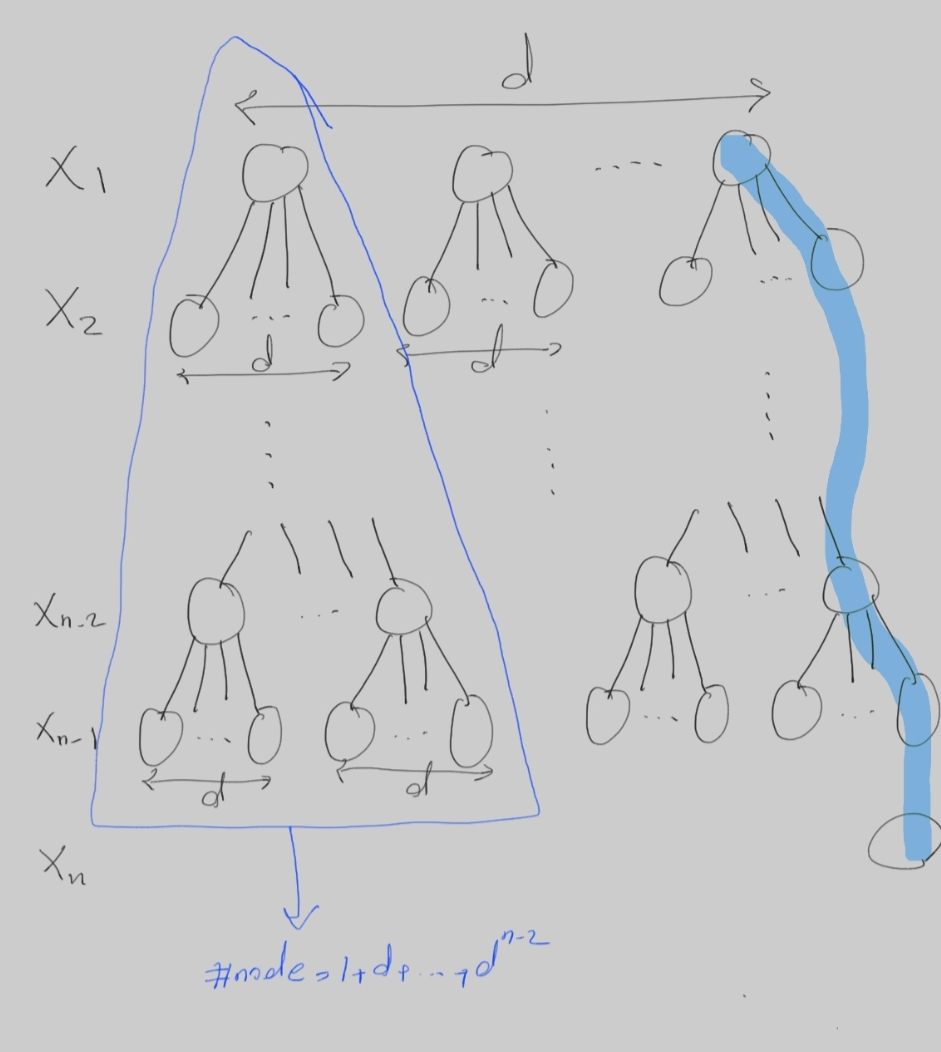
\includegraphics[width=0.8\textwidth]{backtrack.jpg}
		\caption{حداکثر تعداد بازگشت}
		\label{fig:backtrack}
	\end{figure}
	\end{enumerate}
\end{document}



